\documentclass[]{article}

%%%%%%%%%%%%%%%%%%%
% Packages/Macros %
%%%%%%%%%%%%%%%%%%%
\usepackage{amssymb,latexsym,amsmath,graphicx}     % Standard packages


%%%%%%%%%%%
% Margins %
%%%%%%%%%%%
\addtolength{\textwidth}{1.0in}
\addtolength{\textheight}{1.00in}
\addtolength{\evensidemargin}{-0.75in}
\addtolength{\oddsidemargin}{-0.75in}
\addtolength{\topmargin}{-.50in}


\newtheorem{theorem}{Theorem}
\newenvironment{proof}{\noindent{\bf Proof:}}{$\hfill \Box$ \vspace{10pt}}  


%%%%%%%%%%%%
% Document %
%%%%%%%%%%%%
\begin{document}

\title{Write-up\LaTeX ~File}
\author{Angatvir Sanghera, Tyler Crabtree, Tyler Coy
}
\maketitle

\begin{abstract}
Assignment 3 required us to create an inverted index on our databases which we are able to search through using Whoosh.  
\end{abstract}


\section{Attached Files Summary}
%%%%%%%%%%%%%%%
We have attached all code files remember this was done in Python3. We have also given the SQLite3 database files which were used to create the index. We have also included segment files which are in indexdir.
\subsection{Code File}
There are two code files one of the files is indexer.py This first file takes in the databases and parses our databases and creates an inverted index over it. The second file which is searchEngine.py opens up the documents and does a search over it outputting the results found. 

\section{Team Name}
Dragon Police

\section{Database Schema}
All our database schemas are completely different from one another. Our indexer.py gives the option of declaring our schema's name or going with the default. If default is chosen then the keys are grabbed from the database. We did it this way just in case we wanted to include other databases later. Each of default databases schema's is shown below.
\subsection{Tyler Coy's Schema - dinosaur.db}
Schema(Name=TEXT(stored=True), Description=TEXT(stored=True), Era=TEXT(stored=True), Url=TEXT(stored=True), Image=TEXT(stored=True))

\subsection{Angatvir Sanghera's Schema - mmorpg.db}
Schema(Title=TEXT(stored=True), Status=TEXT(stored=True), Graphics=TEXT(stored=True), Setting=TEXT(stored=True), SubscriptionModel=TEXT(stored=True),\\ InitialReleaseDate=TEXT(stored=True), ServerCloseDate=TEXT(stored=True),\\ Notes=TEXT(stored=True), Description=TEXT(stored=True))

\subsection{Tyler Crabtree's Schema - superfamicom.db}
Schema(Title=TEXT(stored=True), ReleaseDate=TEXT(stored=True),\\ Developer=TEXT(stored=True), Publisher=TEXT(stored=True))

\subsection{Example of choice given}
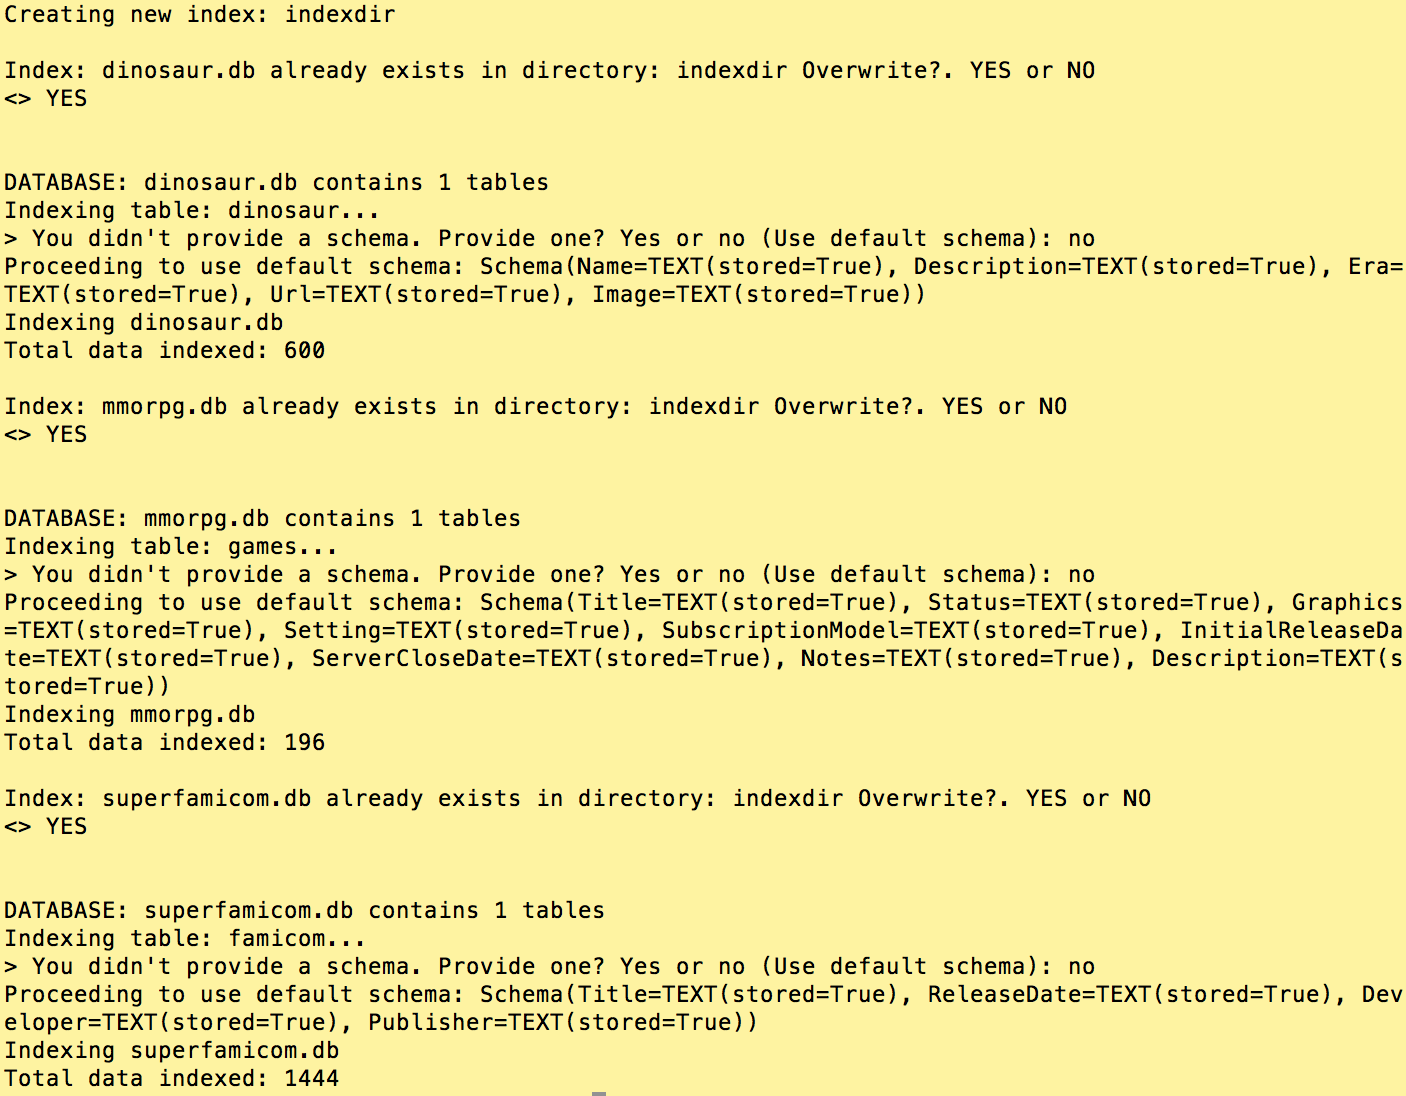
\includegraphics[width=15cm, height=15cm]{schema.png}

\section{Size of Database}
1444 

\section{Searches}
We made our searcher very interactive. You can either search by categories or all categories.

\subsection{Search 1}
Just searched the word hello in the category description\\
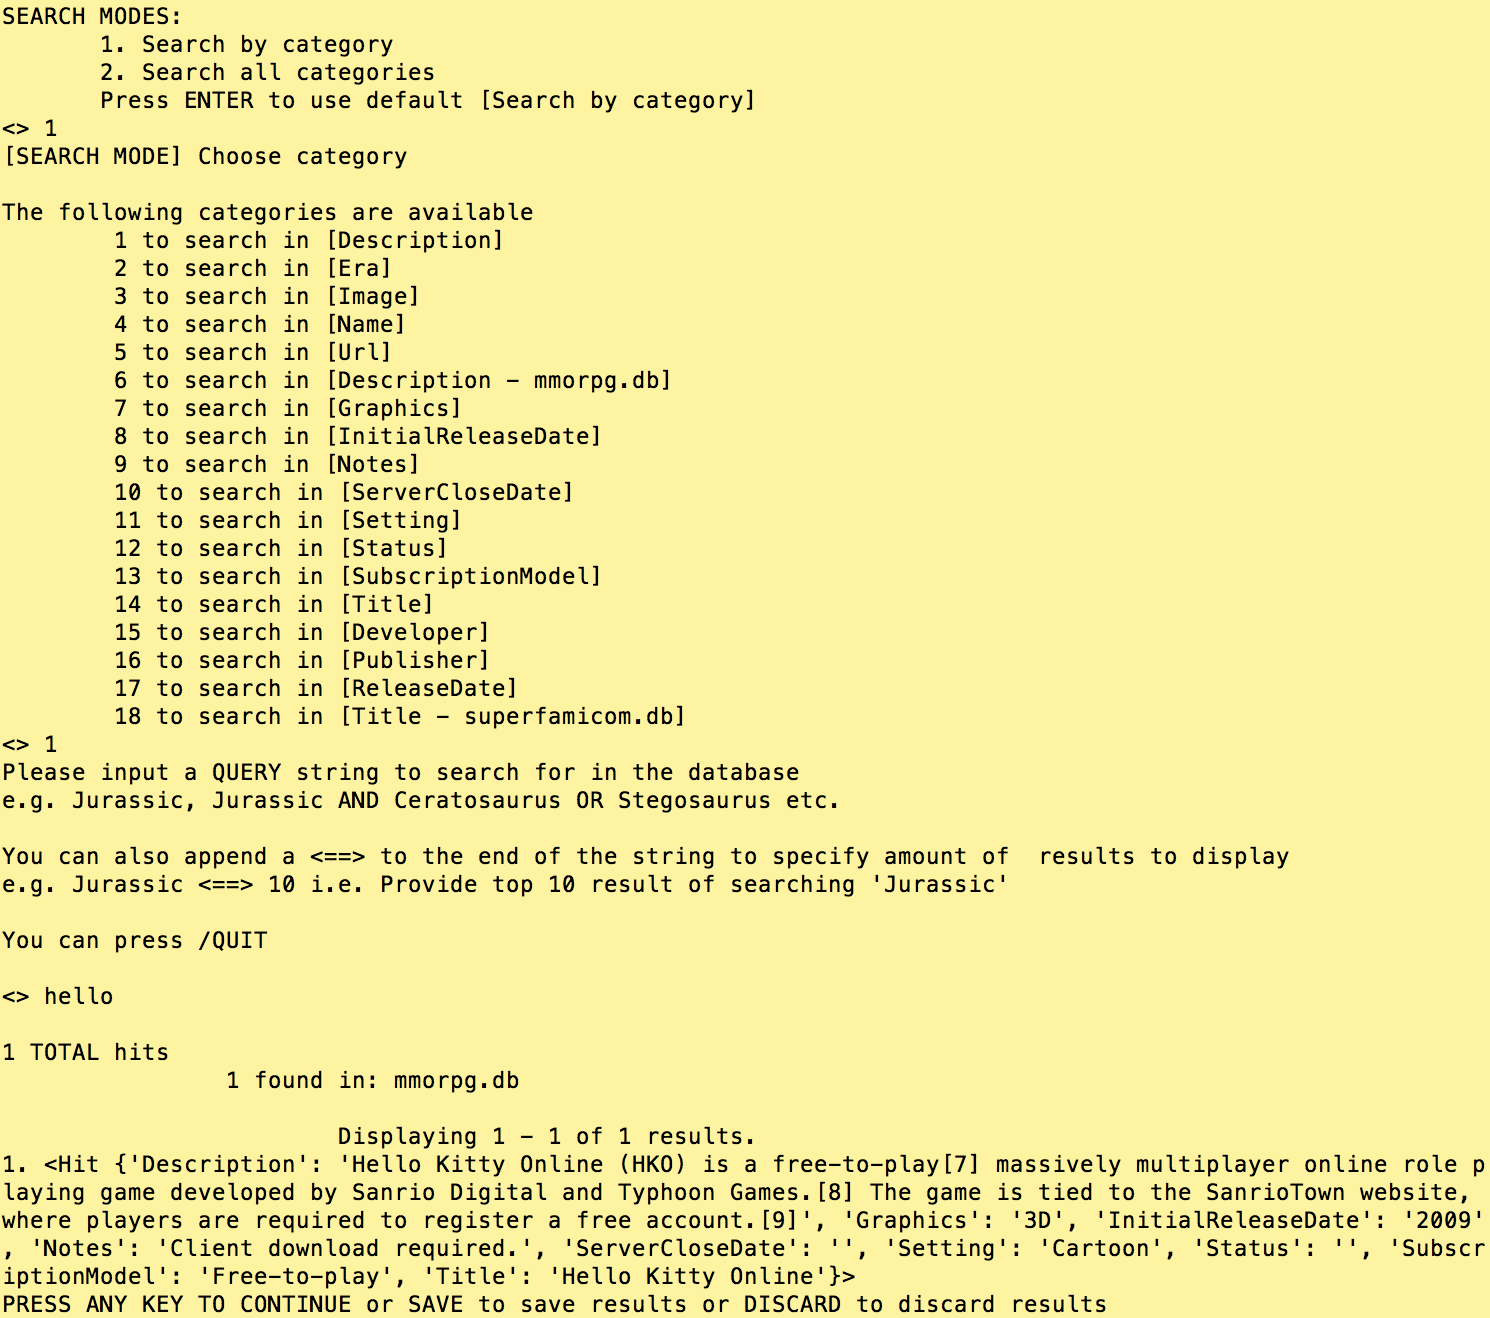
\includegraphics[width=15cm, height=15cm]{search1.png}

\subsection{Search 2}
Just searched Jurassic limiting results to 5\\
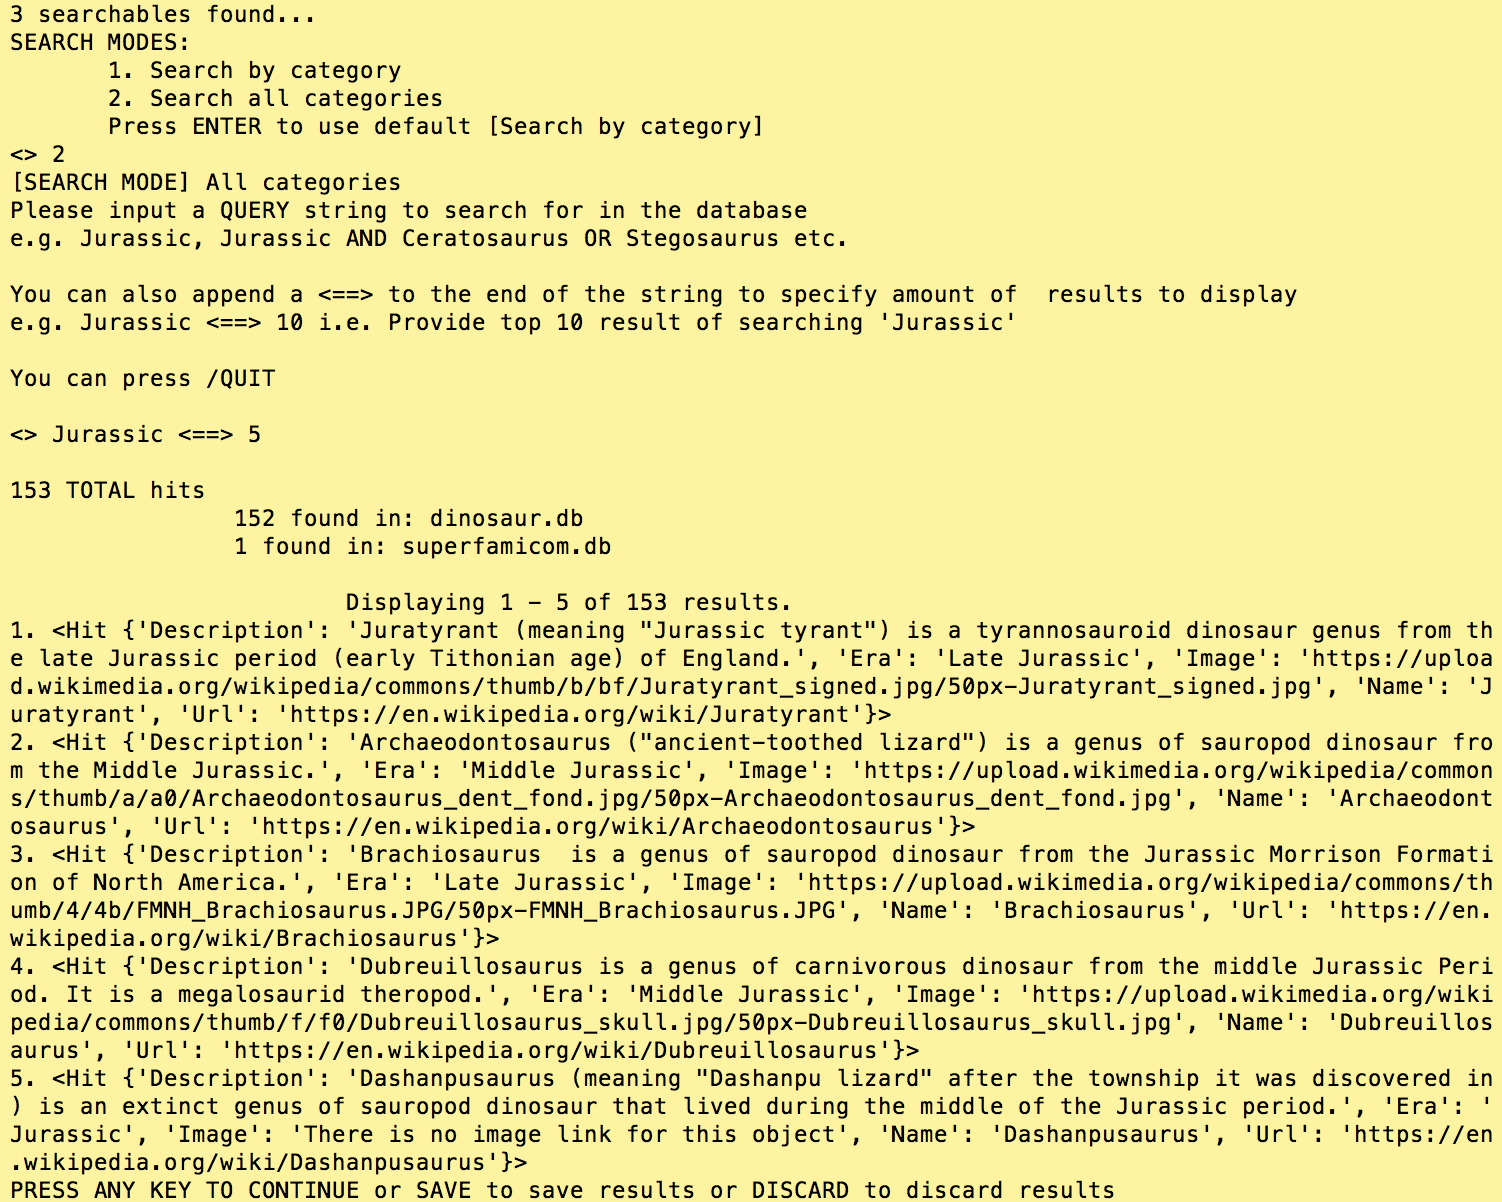
\includegraphics[width=15cm, height=15cm]{search2.png}
\end{document}